\documentclass{article}
\title{Solving the Poisson Equation in Two Dimensional Domain}
\author{Group 5}
\pagestyle{plain}

\usepackage{setspace}
\usepackage{natbib}
\usepackage{algorithm}
\usepackage{graphicx}
\usepackage{amsmath}
\usepackage{amssymb}
\usepackage{tikz}
%\usepackage{algorithmic}
\usepackage{algpseudocode}
%\usepackage{algorithm2e}
\usepackage{geometry}
\usepackage{listings}
\usepackage{array}
\usepackage{hyperref}
\usepackage{float}
\hypersetup{
    colorlinks=true,
    linkcolor=red,
    filecolor=red,      
    urlcolor=red,
    citecolor=red,
}


\geometry{a4paper,left=3.5cm,right=3.5cm,top=3cm,bottom=3cm}

\begin{document}

\maketitle
\normalsize

\section{Introduction}
The Poisson equation is a fundamental partial differential equation (PDE) that models many physical phenomena, including heat distribution, electrostatics, and fluid dynamics. Solving the Poisson equation accurately is crucial for understanding these phenomena in a variety of fields. The objective of this project is to solve the Poisson equation on a rectangular domain using the finite element method (FEM), validate it with an analytical solution, and evaluate the convergence behavior of the numerical solution.

\section{Problem Formulation}
Consider the Poisson equation on the rectangular domain $\Omega=(0,1) \times (0,1)$,
$$
-\Delta u = h, \quad (x, y) \in \Omega.
$$
with the boundary conditions
\begin{align*}
    u = f,\quad& (x, y) \in \partial \Omega_0 \\
\frac{\partial u}{\partial \boldsymbol{n}} = g, \quad& (x, y) \in \partial \Omega_1
\end{align*}
where $\partial \Omega_0 = \{0\} \times [0,1]$, and $\partial \Omega_1 = \partial \Omega - \partial \Omega_0$.
We choose
\begin{align*}
    h \equiv 1, \quad f(y)=0,\quad g(x, y)=0.
\end{align*}
The problems are formulated as the following:
\begin{itemize}
    \item Given mesh sizes of $h=\frac{1}{2^n}$ , perform triangular subdivisions (with equal-sized triangles). For the mesh size of $\frac{1}{3}$, we sketch the diagram. Design a piecewise linear $C^0$ finite element, write a program to solve the problem, and report the computational time. Visualize finite element solutions of mesh size.
    \item Find the analytical solution to the problem, and compute the error between the finite element solution and the analytical solution.
\end{itemize}
\section{Solution Approach}
\section*{1.2 Principle and Algorithm}
We choose

$$
h \equiv 1, \quad f(y)=0\quad g(x, y)=0.
$$

Take the test function $v \in \mathbb{V}:=\left\{v \in \mathbb{H}^{1}(\Omega) \mid v|_{\partial \Omega_{0}}=0\right\}$. Multiply the left-hand side of equation (1.1) by $v$, integrate over $\Omega$, and apply the Gauss-Green formula to obtain

$$
-\int_{\Omega} \Delta u \cdot v=\int_{\Omega} \nabla u \nabla v-\int_{\partial \Omega} \frac{\partial u}{\partial \boldsymbol{n}} \cdot v=\int_{\Omega} \nabla u \nabla v
$$

Thus, the variational form is

\begin{equation*}
\int_{\Omega} \nabla u \nabla v=\int_{\Omega} v
\end{equation*}

The weak solution $u \in \mathbb{V}$ satisfies the above variational form for any $v \in \mathbb{V}$.\\
Similarly, we propose a corresponding functional minimization problem based on the principle of minimum potential energy:

$$
J(u)=\min_{v \in \mathbb{V}} J(v)
$$

where

$$
J(v)=\frac{1}{2} \int_{\Omega}|\nabla v|^{2}-\int_{\Omega} v
$$

This problem is equivalent to the variational form of the original problem.\\
Consider the triangular mesh as shown in Figures \ref{fig:mesh} (element diameter $\frac{1}{3}$) . For convenience, let $h$ denote the element diameter in the mesh, $N$ the number of nodes, and $M$ the number of elements. Then, $N=\frac{1}{h^{2}}+\frac{2}{h}+1$, and $M=\frac{2}{h^{2}}$.

\begin{figure}[h]
    \centering
    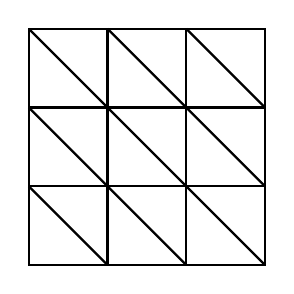
\begin{tikzpicture}[scale=3]
        % Draw the outer square
        \draw[thick] (0, 0) rectangle (1, 1);

        % Draw the grid for the 9 sub-squares
        \draw[thick] (1/3, 0) -- (1/3, 1);
        \draw[thick] (2/3, 0) -- (2/3, 1);
        \draw[thick] (0, 1/3) -- (1, 1/3);
        \draw[thick] (0, 2/3) -- (1, 2/3);

        % Draw the diagonals for each sub-square from bottom right to upper left
        \foreach \i in {0, 1, 2} {
            \foreach \j in {0, 1, 2} {
                \draw[thick] ({(\i+1)/3}, {\j/3}) -- ({\i/3}, {(\j+1)/3}); % Draw diagonal from bottom right to upper left
            }
        }
    \end{tikzpicture}
    \caption{A unit square divided into 9 sub-squares, each subdivided into two triangles.}
    \label{fig:mesh}
\end{figure}

Next, we introduce the $P_1$ Lagrange finite element space as
$$
\mathbb{V}_{h}=\left\{u \in C(\bar{\Omega}): \left.u\right|_{T_{i}} \in \mathbb{P}_{1}\left(T_{i}\right), \forall T_{i} \in \mathcal{T}_{h}(\Omega)\right\}
$$

We then take the finite element trial function space and test function space as

$$
\mathbb{V}_{h}\left(0 ; \Omega_{0}\right)=\left\{u \in \mathbb{V}_{h}: u\left(A_{i}\right)=0, \forall A_{i} \in \partial \Omega_{0}\right\}
$$

For the variational form (1.2), we obtain the finite element problem

\[
\left\{\begin{array}{l}
\text { Find } u_{h} \in \mathbb{V}_{h}\left(0 ; \Omega_{0}\right), \text { such that }  \tag{1.3}\\
a\left(u_{h}, v_{h}\right)=F\left(v_{h}\right), \quad \forall v_{h} \in \mathbb{V}_{h}\left(0 ; \Omega_{0}\right) .
\end{array}\right.
\]

where

$$
a(u, v)=\int_{\Omega} \nabla u \nabla v, \quad F(v)=\int_{\Omega} v.
$$

Let $\varphi_{i} \in \mathbb{V}_{h}$ satisfy

$$
\varphi_{i}\left(A_{j}\right)=\delta_{i j}, \quad i=1,2, \dots, N
$$

Where $A_{j}$ are the nodes of the mesh. Then, $\left\{\varphi_{i}\right\}_{i=1}^{N}$ forms a basis for $\mathbb{V}_{h}$, and $\left\{\varphi_{i}\right\}_{A_{i} \notin \partial \Omega_{0}}$ forms a basis for $\mathbb{V}_{h}\left(0 ; \Omega_{0}\right)$. Let

$$
u_{h}=\sum_{j=1}^{N_{h}} u_{j} \varphi_{j}, \quad v_{h}=\sum_{i=1}^{N_{h}} v_{i} \varphi_{i}
$$

where $N_{h}=\frac{1}{h^{2}}+\frac{1}{h}$. The discrete problem (1.3) is equivalent to

$$
\sum_{j=1}^{N_{h}} a\left(\varphi_{j}, \varphi_{i}\right) u_{j}=F\left(\varphi_{i}\right), \quad i=1,2, \dots, N_{h}
$$

i.e.,

\begin{equation}
\boldsymbol{K} \boldsymbol{u}_{h}=\boldsymbol{f} \label{eq:stiff}
\end{equation}

When computing the stiffness matrix $\boldsymbol{K}$ and load vector $\boldsymbol{f}$, we calculate the element stiffness matrix $\boldsymbol{K}^{e}$ and element load vector $\boldsymbol{f}^{e}$ by scanning the elements. The algorithm is as follows:

\begin{algorithm}
\caption{Algorithm for forming the stiffness matrix and load vector}
\begin{algorithmic}

\State \textbf{Input:} $\boldsymbol{K} = (k(i, j)) := 0$, $\boldsymbol{f} = (f(i)) := 0$
\For{$e = 1$ to $M$}
    \State Compute element stiffness matrix $\boldsymbol{K}^{e} = \left(k^{e}(\alpha, \beta)\right)$
    \State Compute element load vector $\boldsymbol{f}^{e} = \left(f^{e}(\alpha)\right)$
    \For{each $\alpha, \beta$}
        \State $k(e n(\alpha, e), e n(\beta, e)) = k(e n(\alpha, e), e n(\beta, e)) + k^{e}(\alpha, \beta)$
        \State $f(e n(\alpha, e)) = f(e n(\alpha, e)) + f^{e}(\alpha)$
    \EndFor
\EndFor
\State \textbf{Output:} $\boldsymbol{K}$, $\boldsymbol{f}$
\end{algorithmic}
\end{algorithm}

Where $en(\alpha,e)$ denotes the assigned number of triangular nodes (global)If the coordinates of the three vertices of element $T_{e}$ are $\boldsymbol{A}_{1}^{e}=\left(x_{1}, y_{1}\right)^{T}, \boldsymbol{A}_{2}^{e}=\left(x_{2}, y_{2}\right)^{T}, \boldsymbol{A}_{3}^{e}=\left(x_{3}, y_{3}\right)^{T}$, then the affine transformation $\boldsymbol{x}=L_{e}(\hat{\boldsymbol{x}})=\boldsymbol{A}_{e} \hat{\boldsymbol{x}}+\boldsymbol{a}_{e}$ maps the reference triangle $T_{s}$ to $T_{e}$, where

$$
\boldsymbol{A}_{e}=\left(\boldsymbol{A}_{2}^{e}-\boldsymbol{A}_{1}^{e}, \boldsymbol{A}_{3}^{e}-\boldsymbol{A}_{1}^{e}\right), \quad \boldsymbol{a}_{e}=\boldsymbol{A}_{1}^{e} .
$$

The element stiffness matrix is

$$
\boldsymbol{K}^{e}=\frac{1}{2 \operatorname{det} \boldsymbol{A}_{e}}\left(\begin{array}{ll}
y_{2}-y_{3} & x_{2}-x_{3} \\
y_{3}-y_{1} & x_{3}-x_{1} \\
y_{1}-y_{2} & x_{1}-x_{2}
\end{array}\right)\left(\begin{array}{ccc}
y_{2}-y_{3} & y_{3}-y_{1} & y_{1}-y_{2} \\
x_{2}-x_{3} & x_{3}-x_{1} & x_{1}-x_{2}
\end{array}\right)
$$
The element load vector is given by

$$
\boldsymbol{f}^{e}=\frac{\operatorname{det} \boldsymbol{A}_{e}}{6}\left(\begin{array}{l}
1 \\
1 \\
1
\end{array}\right).
$$

Also note that

$$
\operatorname{det} \boldsymbol{A}_{e}=2\left|T_{e}\right|=h^{2}
$$

Thus, we can calculate the stiffness matrix \( \boldsymbol{K} \) and the load vector \( \boldsymbol{f} \), and then solve equation \eqref{eq:stiff} to obtain the finite element solution \( u_{h} \).
\subsection{Analytic Solution}
Under the chosen conditions of \( f, g, h \), the original problem becomes

\[
\begin{cases}-u_{x x}-u_{y y}=1, & (x, y) \in \Omega  \\ u(0, y)=0, & y \in[0,1] \\ u_{y}(x, 0)=u_{y}(x, 1)=0, & x \in[0,1] \\ u_{x}(1, y)=0, & y \in[0,1]\end{cases}
\]

Next, we will find the analytical solution of equation (1.5) using the method of separation of variables.\\
Consider a non-zero solution of the form of separation of variables

$$
u(x, y)=X(x) Y(y)
$$

Substituting it into the homogeneous equation

$$
u_{x x}+u_{y y}=0, \quad(x, y) \in \Omega,
$$

we obtain

$$
X^{\prime \prime}(x) Y(y)+X(x) Y^{\prime \prime}(y)=0, \quad(x, y) \in \Omega
$$

which implies

$$
\frac{X^{\prime \prime}(x)}{X(x)}=-\frac{Y^{\prime \prime}(y)}{Y(y)} .
$$

In the above equation, the left side is a function of \( x \), and the right side is a function of \( y \); hence they can only be equal to a constant, denoted by \( \lambda \). Thus, we have

$$
\begin{array}{ll}
X^{\prime \prime}(x)-\lambda X(x)=0, & x \in(0,1) \\
Y^{\prime \prime}(y)+\lambda Y(y)=0, & y \in(0,1)
\end{array}
$$

Substituting \( u(x, y) \) into the homogeneous boundary conditions

$$
u_{y}(x, 0)=u_{y}(x, 1)=0, \quad x \in[0,1]
$$

gives us

$$
X(x) Y^{\prime}(0)=X(x) Y^{\prime}(1)=0, \quad x \in[0,1]
$$

Since \( u(x, y) \not \equiv 0 \), we have \( X(x) \not \equiv 0 \), leading to

$$
Y^{\prime}(0)=Y^{\prime}(1)=0 .
$$

Thus, we obtain the Sturm-Liouville boundary value problem

$$
\left\{\begin{array}{l}
Y^{\prime \prime}(y)+\lambda Y(y)=0, \quad y \in(0,1) \\
Y^{\prime}(0)=Y^{\prime}(1)=0
\end{array}\right.
$$

The characteristic values of this problem are given by

$$
\lambda_{n}=(n \pi)^{2}, \quad n=0,1, \cdots,
$$

with the corresponding eigenfunctions being

$$
Y_{n}(y)=\cos n \pi y, \quad n=0,1, \cdots
$$

Returning to the original problem, we express the solution \( u(x, y) \) in terms of the eigenfunction series \( \{\cos n \pi y\}(n=0, 1, \cdots) \):

$$
u(x, y)=\sum_{n=0}^{\infty} X_{n}(x) \cos n \pi y.
$$

Substituting these expressions into the original problem and using the completeness of the eigenfunction series \( \{\cos n \pi y\}(n=0,1,\cdots) \), we obtain that \( X_{n}(x) \) satisfies the following ordinary differential equations:

$$
\begin{aligned}
& \left\{\begin{array}{l}
X_{0}^{\prime \prime}(x)=-1, \quad x \in(0,1), \\
X_{0}(0)=0, X_{0}^{\prime}(1)=0 .
\end{array}\right.\\
& \left\{\begin{array}{l}
X_{n}^{\prime \prime}(x)-(n \pi)^{2} X_{n}(x)=0, \quad x \in(0,1), \quad(n \geq 1) \\
X_{n}(0)=0, X_{n}^{\prime}(1)=0 .
\end{array}\right.
\end{aligned}
$$

Solving gives us

$$
X_{0}(x)=-\frac{x^{2}}{2}+x.
$$

Thus, the analytical solution of equation (1.5) is

\begin{equation*}
u(x, y)=-\frac{x^{2}}{2}+x.
\end{equation*}

Restricting the analytical solution (1.6) to the grid points of the corresponding triangular mesh yields a vector \( u \), which can be compared with the computed solution \( u_{h} \). The \( \mathbb{L}^{\infty} \) error of the finite element solution can be approximated by calculating \( \left\|u-u_{h}\right\|_{\infty} \).


% {\color{blue}More to add: Introduction to the problem (why should we study this problem), tag this latex file into the git repo, write expected outcome, make sure this compiles outside of overleaf}

\vspace{5mm}

A brief procedure on how to do coding:
\begin{figure}[H]
    \centering
\includegraphics[scale=0.2]{IMG_9C01D8EECCB6-1.jpeg}
    % \caption{Caption}
    % \label{fig:enter-label}
\end{figure}

\section{Implementation Plan}
We will implement this problem using C++ with the following steps:
\begin{itemize}
    \item \textbf{Project Structure:} Organize code into folders for sources, inputs, tests, and documentation. Use a \texttt{Makefile} to streamline building and linking.

    \item \textbf{Input Parsing:} Configure parameters (e.g., mesh size, boundary conditions) via an INI-style file. Libraries like \texttt{libGRVY} support flexible parsing and backward compatibility.

    \item \textbf{Algorithm Implementation:} Develop the FEM algorithm with:
    \begin{itemize}
        \item \textbf{Mesh generation:} Triangular subdivision based on specified mesh sizes.
        \item \textbf{Stiffness matrix and load vector assembly.}
        \item \textbf{Boundary conditions:} Apply Dirichlet and Neumann conditions as specified.
    \end{itemize}

    \item \textbf{Performance Timing:} Use \texttt{libGRVY} to time sections of code for performance insights.

    \item \textbf{Testing:} Build a test suite to validate functionality (unit, integration, and regression tests). Use \texttt{Boost.Test} or \texttt{Bats} for script testing.

    \item \textbf{Logging and Documentation:} Integrate logging to aid debugging and add a \texttt{README} with setup and usage instructions.
\end{itemize}

\section{Expected Outcome}
This implementation is expected to yield
\begin{itemize}
    \item \textbf{Accurate Numerical Solution:} A finite element solution that approximates the analytical solution for the Poisson equation on a rectangular domain, with error metrics quantifying accuracy.

    \item \textbf{Convergence Analysis:} Demonstration of convergence through error reduction as mesh sizes decrease, validating the FEM approach.

    \item \textbf{Performance Benchmarks:} Timing data for key algorithm stages (e.g., matrix assembly, solution computation) to assess the solver's efficiency and identify performance bottlenecks.

    \item \textbf{Automated Testing Results:} Validation of implementation correctness and robustness through unit, integration, and regression tests, increasing reliability for scientific computing applications.

\end{itemize}


%\bibliographystyle{plain}
%\bibliography{ref_twoscale}



















\end{document}

%%\begin{figure}[H]
    \centering
    \includegraphics[scale=0.7]{spline1.png}
    \caption{插值函数随着插值点增多的表现}
    \label{}
\end{figure}
三种求积方法的实现}